ثابت کنید 
$$f^{3}(x_{0}) = \frac{5f(x_{0}) - 18f(x_{0} - h) + 24f(x_{0} - 2h) - 14f(x_{0} -3h) + 3f(x_{0} - 4h)}{2h^{3}} + O(h^{2})$$

راهنمایی: از بسط تیلور استفاده کنید.


پاسخ:


مانند شکل زیر می‌توان عمل کرد.

\begin{center}
    \begin{figure}[H]
        \centering
        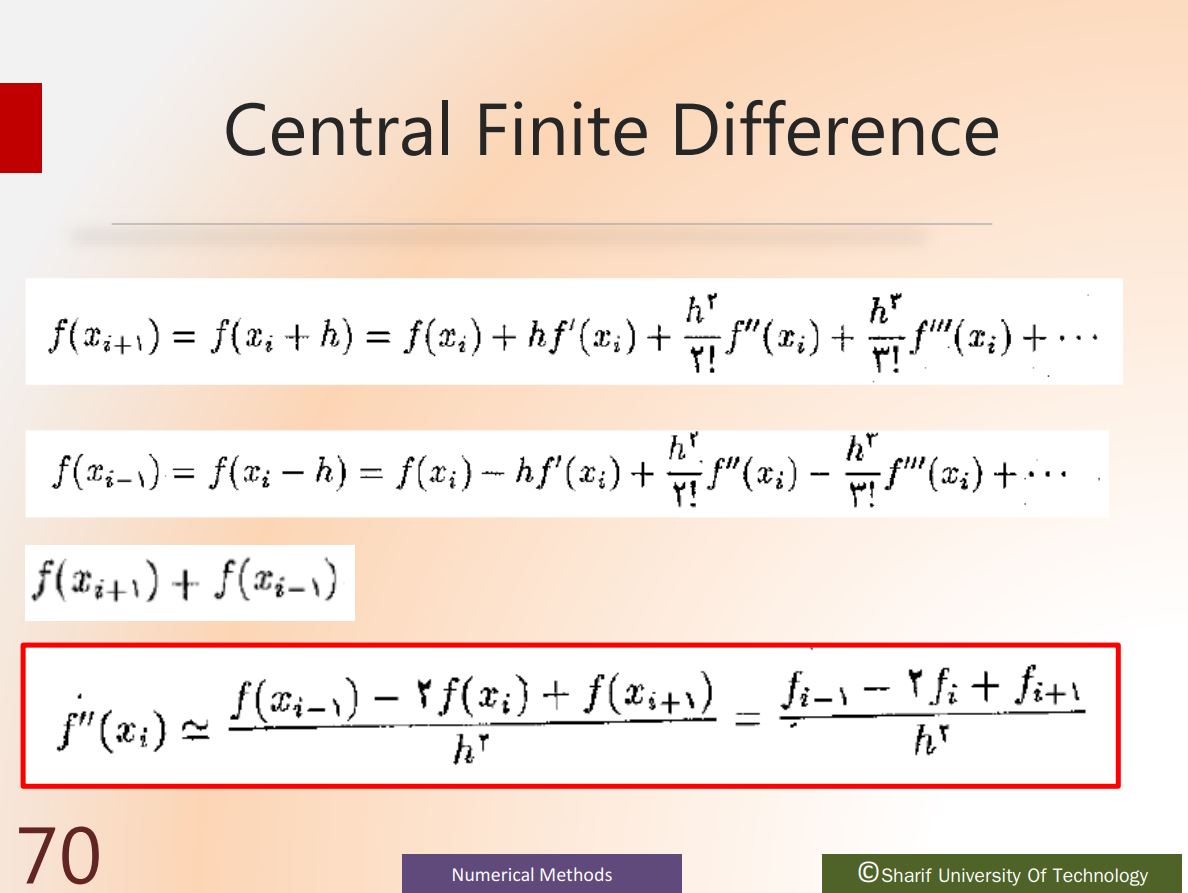
\includegraphics[width=0.8\linewidth]{q5.JPG}
        \caption{راه حل برای مسئله ساده‌تر}
        \label{fig:1}
    \end{figure}
\end{center}